\chapter{O jogo dos colegas de quarto}

Vimos que a assimetria de informação pode levar o jogo a um resultado que não é ótimo para nenhum dos jogadores, onde um jogador é capaz de, até mesmo, aumentar seu pagamento ao mudar de estratégia unilateralmente. É de nosso interesse saber se esse também o caso quando jogo se repete ao longo do tempo, sendo regido pela equação $\eqref{defEqRepHR}$, onde esperamos que os jogadores sejam capazes de identificar explorar as hiperpreferências dos demais. Para fazer essa análise, vamos definir o jogo dos colegas de quarto, onde podemos observar como o conflito de interesses e preferências interfere no perfil de estratégias ao longo do tempo. É importante ressaltar que este jogo ainda é como nos jogos clássicos, onde a cada instante dois jogadores vizinhos são selecionados de maneira aleatória para jogar entre si e os jogadores selecionados irão jogar uma estratégia pura com uma dada probabilidade. Dito isso, nós usaremos uma analogia com a rotina de colegas de quarto para que o jogo fique mais fácil de ser interpretado, mesmo que ela possa perder um pouco o seu sentido se pensarmos na forma como ocorrem os encontros entre jogadores em jogos evolucionários.

Neste jogo temos três jogadores em um grafo completo, um triângulo no qual todos interagem entre si, onde os jogadores são colegas de quarto, porém existem sentimentos não correspondidos que mudam a forma como eles interagem. Para ilustrar essa dinâmica vamos considerar duas estratégias, ser $\textit{organizado}$ e ser $\textit{desordeiro}$, ou $O$ e $D$. Consideramos que cada um possui sua própria matriz de pagamentos, definidas abaixo. Lembre-se que a entrada $b_{k,i,j}$ da matriz $B_k$ é o pagamento do jogador $k$ ao usar a estratégia $i$ contra a estratégia $j$, com $k\in\{u,v,w\}$ e $i,j\in\{O,D\}$, neste caso.

\begin{equation}
    \label{payoffLoveTri}
    B_u=
    \begin{bmatrix}
        0 & 1\\ 
        0 & 0 
    \end{bmatrix},
    B_v=
    \begin{bmatrix}
        0 & 0\\ 
        1 & 0 
    \end{bmatrix},
    B_w=
    \begin{bmatrix}
        1 & 0\\ 
        0 & 0 
    \end{bmatrix}
\end{equation}

Note que $u$ e $v$ se complementam, pois $u$ só possui pagamento ao jogar $O$ com alguém que jogue $D$ e $v$ só possui pagamento ao jogar $D$ para alguém que jogue $O$, enquanto $w$ só se beneficia ao jogar $O$ contra $O$. Assim, com jogadores racionais, é esperado que o perfil $(e_1,e_2,e_1)$ seja o resultado final do jogo, onde $u$ e $v$ irão se relacionar de maneira complementar, $v$ receberá um pagamento de ambas suas relações e $w$ irá conseguir algum benefício apenas de sua relação com $u$.

Este jogo se torna interessante ao considerarmos jogadores hiper-racionais, pois as interações entre eles deixam de ser tão óbvias. Considere o caso no qual o jogador $u$ possui sentimentos por $v$, $v$ possui sentimentos por $w$ que, por sua vez, possui somente amor próprio. Essas relações podem ser representadas através da seguinte matriz de preferências.
\begin{equation}
    \label{prefPosLoveTri1}
    \Rc=
    \begin{bmatrix}
        \frac{1}{2} & \frac{1}{2} & 0\\ 
        0 & \frac{3}{5} & \frac{2}{5} \\
        0 & 0 & 1
    \end{bmatrix}
\end{equation}

Assim, as equações de replicação de cada jogador serão como segue.

\begin{equation}
    \label{EqRepLoveTri1}
    \left\{\begin{matrix*}[l]
        \dot{x}_{u,O}=x_{u,O}(1-x_{u,O})\left(\frac{3}{4}x_{v,D}+\frac{1}{4}x_{w,D}\right) \\
        \dot{x}_{v,O}=x_{v,O}(1-x_{v,O})\left(-\frac{3}{10}x_{u,O}-\frac{1}{10}x_{w,O}\right) \\
        \dot{x}_{w,O}=x_{w,O}(1-x_{w,O})\left(\frac{1}{2}x_{u,O}+\frac{1}{2}x_{v,O}\right)
    \end{matrix*}\right.
\end{equation}

Pelas equações, podemos concluir que o resultado será o mesmo do jogo clássico, o perfil de estratégias $(e_1,e_2,e_1)$. Isso pode ser observado na figura \ref{fig:love_tri1.png}.

\begin{figure}[h]
    \caption{Evolução do uso da estratégia $O$ para cada um dos colegas de quarto com $\Rc$ dada em $\eqref{prefPosLoveTri1}$,  $[0.5 \; 0.5]^T$ como condição inicial para todos jogadores e $t\in[0,40]$.}
    \centerline{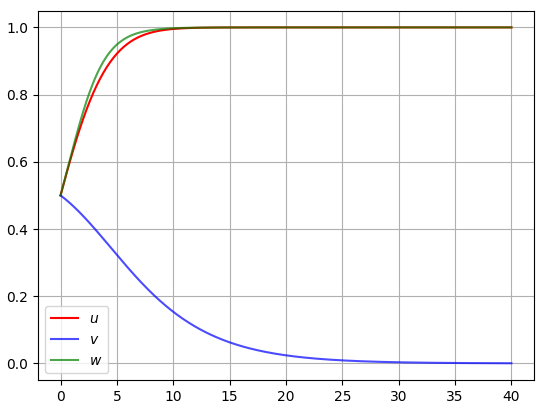
\includegraphics[scale=0.8]{./img/love_tri1.png}}
    \label{fig:love_tri1.png}
\end{figure}

Para tornar o jogo mais interessante vamos supor que a afeição de $v$ por $w$ esteja cada vez maior e, com isso, $v$ passe a valorizá-lo com a mesma intensidade que valoriza a si mesmo. Por conta disso, $u$ começa a desconfiar dos sentimentos de $v$ por $w$ e, por ciúmes, passa a querer o prejuízo de $w$. Essa nova dinâmica pode ser representada pela seguinte matriz de preferências.

\begin{equation}
    \label{prefPosLoveTri2}
    \Rc=
    \begin{bmatrix}
        \frac{2}{5} & \frac{2}{5} & -\frac{1}{5}\\ 
        0 & \frac{1}{2} & \frac{1}{2} \\
        0 & 0 & 1
    \end{bmatrix}
\end{equation}

Com essas mudanças, as equações $\eqref{EqRepLoveTri1}$ serão dadas por
\begin{equation}
    \label{EqRepLoveTri2}
    \left\{\begin{matrix*}[l]
        \dot{x}_{u,O}=x_{u,O}(1-x_{u,O})\left(\frac{2}{5}x_{v,D}+\frac{1}{5}x_{w,D} -\frac{1}{10}x_{w,O}\right) \\
        \dot{x}_{v,O}=x_{v,O}(1-x_{v,O})\left(\frac{1}{4}x_{w,O}-\frac{1}{4}x_{u,O}\right) \\
        \dot{x}_{w,O}=x_{w,O}(1-x_{w,O})\left(\frac{1}{2}x_{u,O}+\frac{1}{2}x_{v,O}\right)
    \end{matrix*}\right.
\end{equation}

Note que a equação de $w$ não mudou e, portanto, se $x_{u,O}>0$ ou $x_{v,O}>0$ teremos que $x_{w,O}\to 1$. Então, assumindo que $x_{w,O}=1$ enquanto $x_{u,O},x_{v,O}\in(0,1)$ para algum $t>0$ , temos que
\begin{equation}
    \label{uDedicav}
    \dot{x}_{u,O}>0 \Longleftrightarrow x_{v,O} \leq \frac{3}{4},
\end{equation}
ou seja, uma condição para que $u$ continue jogando $O$ e agradando ao jogador $v$. Porém, ao mesmo tempo, temos
\begin{equation}
    \label{vDedicau}
    \dot{x}_{v,O} \leq 0 \Longleftrightarrow x_{u,O} \geq x_{w,O},
\end{equation}
que nos dá uma condição para que $v$ não deixe de jogar $D$, que agrada o jogador $u$, para jogar $O$, que agrada o jogador $w$. Caso as condições $\eqref{uDedicav}$ e $\eqref{vDedicau}$ não sejam satisfeitas, teremos como solução o perfil de estratégias $(e_2,e_1,e_1)$, onde $u$ passa a jogar $D$ apenas para diminuir o pagamento de $w$, pois ele não recebe mais nenhum benefício de sua relação com $v$, que agora joga $O$ para aumentar o pagamento de $w$, mesmo não recebendo nenhum pagamento efetivo dessa relação. Essa dinâmica pode ser observada na figura \ref{fig:love_tri2.png}.

\begin{figure}[h]
    \caption{Evolução do uso da estratégia $O$ para cada um dos colegas de quarto com $\Rc$ dada em $\eqref{prefPosLoveTri2}$,  $[0.5 \; 0.5]^T$ como condição inicial para todos jogadores e $t\in[0,120]$.}
    \centerline{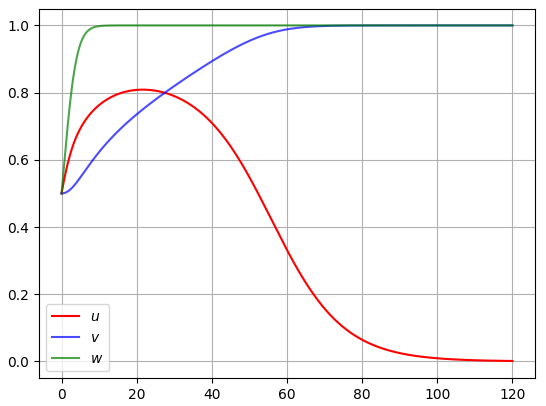
\includegraphics[scale=0.8]{./img/love_tri2.png}}
    \label{fig:love_tri2.png}
\end{figure}

Apesar de parecer simples, essa dinâmica entre colegas de quarto $\textit{organizados}$ e $\textit{desordeiros}$ pode se tornar complicada quando inserimos os sentimentos humanos como variáveis. Neste exemplo conseguimos modelar afeição e ciúmes através das hiperpreferências dos jogadores, exemplificando o que foi dito no capítulo \ref{chap:hiperRacionalidade} e mostrando como a hipótese de racionalidade não é suficiente para modelar o comportamento humano em todas situações.